

\tikzset{every picture/.style={line width=0.75pt}} %set default line width to 0.75pt        
\resizebox{\textwidth}{!}{%
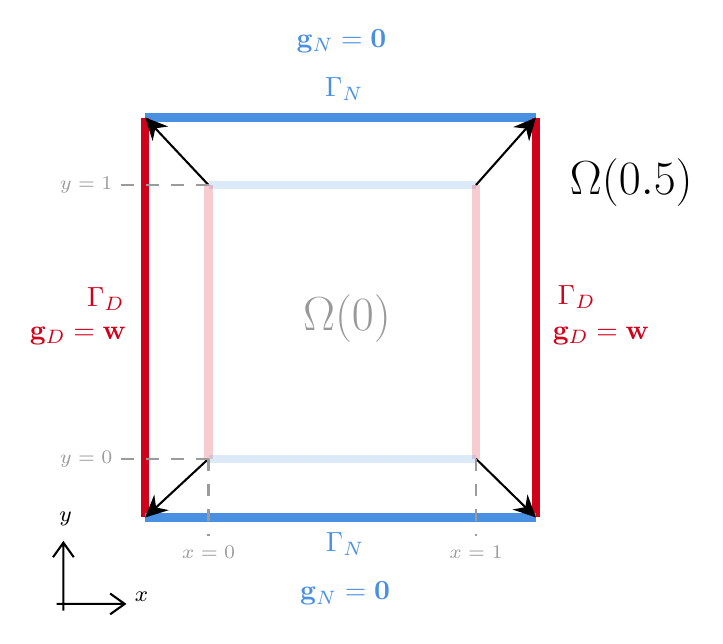
\begin{tikzpicture}[x=0.75pt,y=0.75pt,yscale=-1,xscale=1]
%uncomment if require: \path (0,350); %set diagram left start at 0, and has height of 350

%Straight Lines [id:da3911785235524641] 
\draw [color={rgb, 255:red, 74; green, 144; blue, 226 }  ,draw opacity=1 ][line width=3]    (98.78,72.15) -- (287,72.15) ;
%Straight Lines [id:da08153744945246588] 
\draw [color={rgb, 255:red, 208; green, 2; blue, 27 }  ,draw opacity=1 ][line width=3]    (287,72.15) -- (287,264.82) ;
%Straight Lines [id:da5688674307213424] 
\draw [color={rgb, 255:red, 208; green, 2; blue, 27 }  ,draw opacity=1 ][line width=3]    (98.78,72.15) -- (98.78,264.82) ;
%Straight Lines [id:da13408740199002578] 
\draw [color={rgb, 255:red, 74; green, 144; blue, 226 }  ,draw opacity=1 ][line width=3]    (287,264.82) -- (98.78,264.82) ;
%Straight Lines [id:da8870048899559595] 
\draw [color={rgb, 255:red, 74; green, 144; blue, 226 }  ,draw opacity=0.2 ][line width=3]    (129.28,104.65) -- (258.14,104.65) ;
%Straight Lines [id:da8723650118672401] 
\draw [color={rgb, 255:red, 208; green, 2; blue, 27 }  ,draw opacity=0.2 ][line width=3]    (258.14,104.65) -- (258.14,236.55) ;
%Straight Lines [id:da4357741269330557] 
\draw [color={rgb, 255:red, 208; green, 2; blue, 27 }  ,draw opacity=0.2 ][line width=3]    (129.28,104.65) -- (129.28,236.55) ;
%Straight Lines [id:da9191492030234965] 
\draw [color={rgb, 255:red, 74; green, 144; blue, 226 }  ,draw opacity=0.2 ][line width=3]    (258.14,236.55) -- (129.28,236.55) ;
%Shape: Axis 2D [id:dp9350720821526224] 
\draw  (56.08,306.48) -- (88.88,306.48)(59.36,276.96) -- (59.36,309.76) (81.88,301.48) -- (88.88,306.48) -- (81.88,311.48) (54.36,283.96) -- (59.36,276.96) -- (64.36,283.96)  ;

%Straight Lines [id:da021521710554898155] 
\draw    (129.28,104.65) -- (100.83,74.34) ;
\draw [shift={(98.78,72.15)}, rotate = 46.82] [fill={rgb, 255:red, 0; green, 0; blue, 0 }  ][line width=0.08]  [draw opacity=0] (10.72,-5.15) -- (0,0) -- (10.72,5.15) -- (7.12,0) -- cycle    ;
%Straight Lines [id:da8341315604563517] 
\draw    (258.14,104.65) -- (285.01,74.39) ;
\draw [shift={(287,72.15)}, rotate = 131.61] [fill={rgb, 255:red, 0; green, 0; blue, 0 }  ][line width=0.08]  [draw opacity=0] (10.72,-5.15) -- (0,0) -- (10.72,5.15) -- (7.12,0) -- cycle    ;
%Straight Lines [id:da6015135889734096] 
\draw    (258.14,236.55) -- (284.86,262.72) ;
\draw [shift={(287,264.82)}, rotate = 224.4] [fill={rgb, 255:red, 0; green, 0; blue, 0 }  ][line width=0.08]  [draw opacity=0] (10.72,-5.15) -- (0,0) -- (10.72,5.15) -- (7.12,0) -- cycle    ;
%Straight Lines [id:da44271674446744247] 
\draw    (129.28,236.55) -- (100.98,262.78) ;
\draw [shift={(98.78,264.82)}, rotate = 317.18] [fill={rgb, 255:red, 0; green, 0; blue, 0 }  ][line width=0.08]  [draw opacity=0] (10.72,-5.15) -- (0,0) -- (10.72,5.15) -- (7.12,0) -- cycle    ;
%Straight Lines [id:da8787304201926478] 
\draw [color={rgb, 255:red, 155; green, 155; blue, 155 }  ,draw opacity=1 ] [dash pattern={on 4.5pt off 4.5pt}]  (129.28,236.55) -- (129.28,273.6) ;
%Straight Lines [id:da19489772630369218] 
\draw [color={rgb, 255:red, 155; green, 155; blue, 155 }  ,draw opacity=1 ] [dash pattern={on 4.5pt off 4.5pt}]  (258.14,236.55) -- (258.14,273.6) ;
%Straight Lines [id:da9299742276817373] 
\draw [color={rgb, 255:red, 155; green, 155; blue, 155 }  ,draw opacity=1 ] [dash pattern={on 4.5pt off 4.5pt}]  (129.28,236.55) -- (86.5,236.55) ;
%Straight Lines [id:da941430709775763] 
\draw [color={rgb, 255:red, 155; green, 155; blue, 155 }  ,draw opacity=1 ] [dash pattern={on 4.5pt off 4.5pt}]  (129.28,104.65) -- (86.5,104.65) ;

% Text Node
\draw (90.32,159.53) node [anchor=east] [inner sep=0.75pt]  [color={rgb, 255:red, 208; green, 2; blue, 27 }  ,opacity=1 ]  {$\Gamma _{D}$};
% Text Node
\draw (296.14,158.64) node [anchor=west] [inner sep=0.75pt]  [color={rgb, 255:red, 208; green, 2; blue, 27 }  ,opacity=1 ]  {$\Gamma _{D}$};
% Text Node
\draw (194.66,65.55) node [anchor=south] [inner sep=0.75pt]  [color={rgb, 255:red, 74; green, 144; blue, 226 }  ,opacity=1 ]  {$\Gamma _{N}$};
% Text Node
\draw (195.09,270.56) node [anchor=north] [inner sep=0.75pt]  [color={rgb, 255:red, 74; green, 144; blue, 226 }  ,opacity=1 ]  {$\Gamma _{N}$};
% Text Node
\draw (91.05,171.56) node [anchor=north east] [inner sep=0.75pt]  [color={rgb, 255:red, 208; green, 2; blue, 27 }  ,opacity=1 ]  {$\mathbf{g}_{D} =\mathbf{w}$};
% Text Node
\draw (293.65,171.56) node [anchor=north west][inner sep=0.75pt]  [color={rgb, 255:red, 208; green, 2; blue, 27 }  ,opacity=1 ]  {$\mathbf{g}_{D} =\mathbf{w}$};
% Text Node
\draw (195.08,294.46) node [anchor=north] [inner sep=0.75pt]  [color={rgb, 255:red, 74; green, 144; blue, 226 }  ,opacity=1 ]  {$\mathbf{g}_{N} =\mathbf{0}$};
% Text Node
\draw (193.35,42.53) node [anchor=south] [inner sep=0.75pt]  [color={rgb, 255:red, 74; green, 144; blue, 226 }  ,opacity=1 ]  {$\mathbf{g}_{N} =\mathbf{0}$};
% Text Node
\draw (195.99,168.97) node  [font=\LARGE,color={rgb, 255:red, 0; green, 0; blue, 0 }  ,opacity=0.4 ]  {$\Omega ( 0)$};
% Text Node
\draw (301.93,103.47) node [anchor=west] [inner sep=0.75pt]  [font=\LARGE,color={rgb, 255:red, 0; green, 0; blue, 0 }  ,opacity=1 ]  {$\Omega ( 0.5)$};
% Text Node
\draw (129.28,277) node [anchor=north] [inner sep=0.75pt]  [font=\scriptsize,color={rgb, 255:red, 155; green, 155; blue, 155 }  ,opacity=1 ]  {$x=0$};
% Text Node
\draw (258.14,277) node [anchor=north] [inner sep=0.75pt]  [font=\scriptsize,color={rgb, 255:red, 155; green, 155; blue, 155 }  ,opacity=1 ]  {$x=1$};
% Text Node
\draw (84.5,236.55) node [anchor=east] [inner sep=0.75pt]  [font=\scriptsize,color={rgb, 255:red, 155; green, 155; blue, 155 }  ,opacity=1 ]  {$y=0$};
% Text Node
\draw (84.5,104.65) node [anchor=east] [inner sep=0.75pt]  [font=\scriptsize,color={rgb, 255:red, 155; green, 155; blue, 155 }  ,opacity=1 ]  {$y=1$};
% Text Node
\draw (92.26,303) node [anchor=west] [inner sep=0.75pt]  [font=\footnotesize]  {$x$};
% Text Node
\draw (60.4,270.55) node [anchor=south] [inner sep=0.75pt]  [font=\footnotesize]  {$y$};


\end{tikzpicture}
}